\section{Introduction to Embedded Linux}

\begin{frame}{Simplified Linux system architecture}
  \begin{center}
    \includegraphics[height=0.8\textheight]{slides/buildroot-yocto-introduction/linux-system-architecture.pdf}
  \end{center}
\end{frame}

\begin{frame}{Overall Linux boot sequence}
  \begin{center}
    \includegraphics[height=0.8\textheight]{slides/buildroot-yocto-introduction/overall-boot-sequence.pdf}
  \end{center}
\end{frame}

\begin{frame}{Embedded Linux work}
  \begin{itemize}
  \item {\bf BSP work}: porting the bootloader and Linux kernel,
    developing Linux device drivers.
  \item {\bf system integration work}: assembling all the user space
    components needed for the system, configure them, develop the
    upgrade and recovery mechanisms, etc.
  \item {\bf application development}: write the company-specific
    applications and libraries.
  \end{itemize}
\end{frame}

\begin{frame}{Complexity of user space integration}
  \begin{center}
    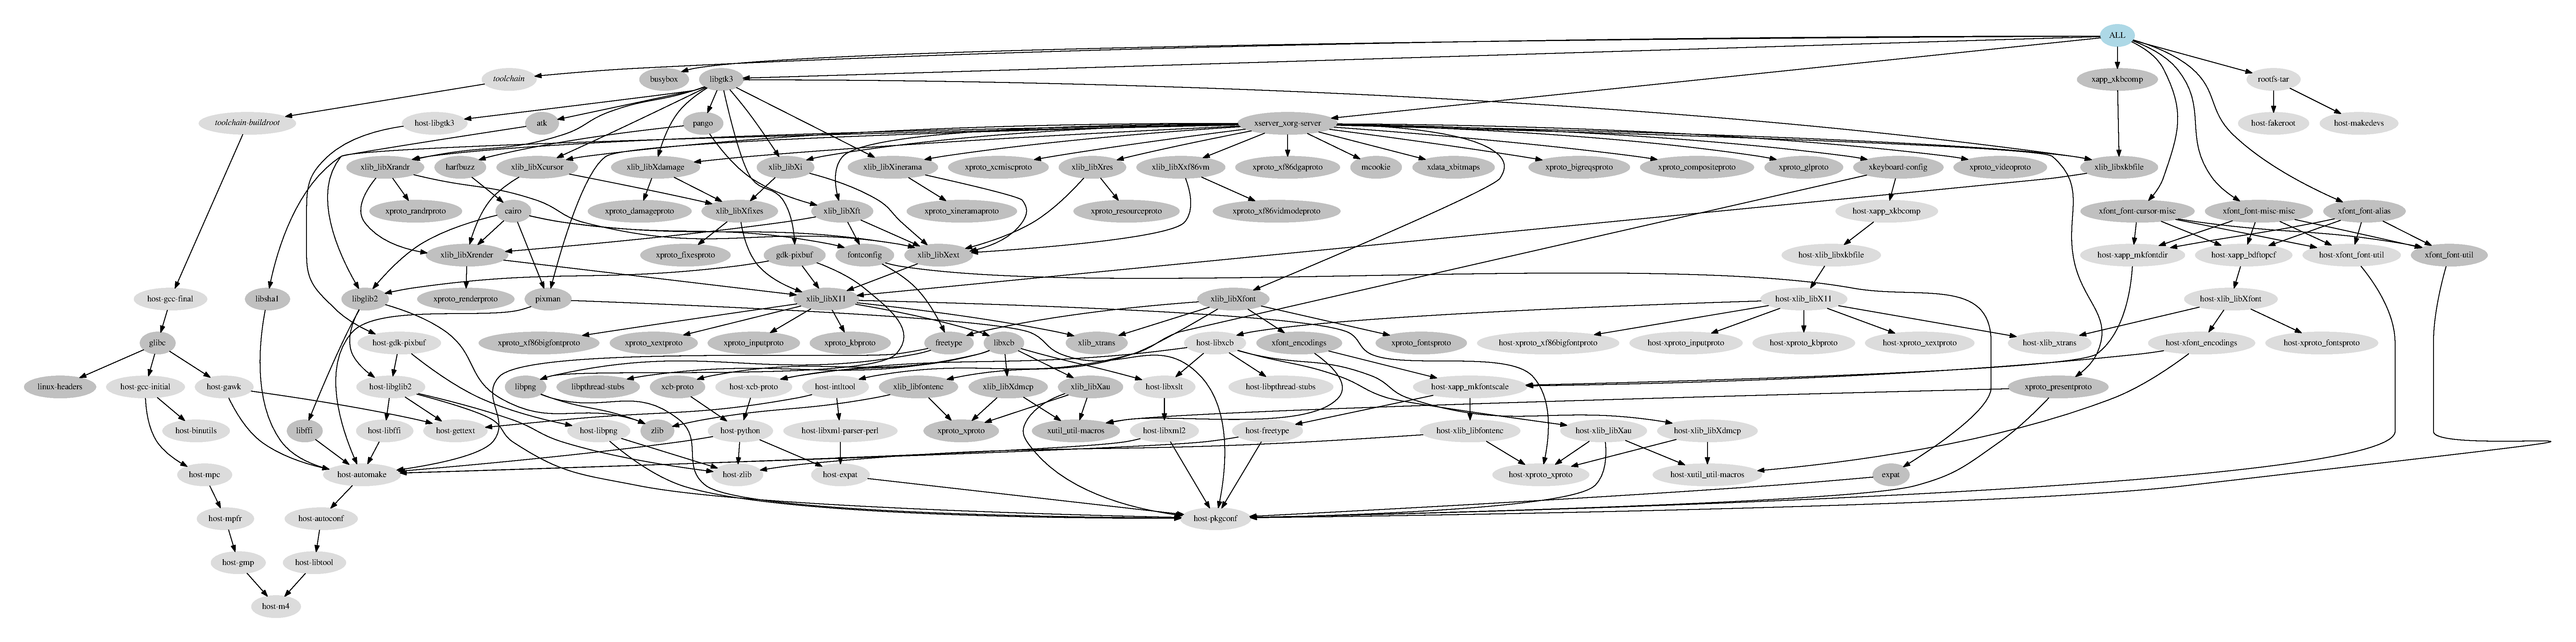
\includegraphics[width=\textwidth]{slides/buildroot-yocto-introduction/graph-depends.pdf}
  \end{center}
\end{frame}

\begin{frame}{System integration: several possibilities}
  \tiny
  \begin{tabularx}{11cm}{|X|X|X|}
    \hline
    & {\bf Pros} & {\bf Cons} \\
    \hline
    {\bf Building everything manually} &
    Full flexibility \newline
    Learning experience &
    Dependency hell \newline
    Need to understand a lot of details \newline
    Version compatibility \newline
    Lack of reproducibility \\
    \hline
    {\bf Binary distribution} \newline Debian, Ubuntu, Fedora, etc.
    &
    Easy to create and extend
    &
    Hard to customize \newline
    Hard to optimize (boot time, size) \newline
    Hard to rebuild the full system from source \newline
    Large system \newline
    Uses native compilation (slow) \newline
    No well-defined mechanism to generate an image \newline
    Lots of mandatory dependencies \newline
    Not available for all architectures \\
    \hline
    {\bf Build systems} \newline Buildroot, Yocto, PTXdist, etc.
    &
    Nearly full flexibility \newline
    Built from source: customization and optimization are easy \newline
    Fully reproducible \newline
    Uses cross-compilation \newline
    Have embedded specific packages not necessarily in desktop distros \newline
    Make more features optional
    &
    Not as easy as a binary distribution \newline
    Build time \\
    \hline
  \end{tabularx}
\end{frame}

\begin{frame}{Embedded Linux build system: principle}
  \begin{center}
    \includegraphics[width=0.9\textwidth]{slides/buildroot-yocto-introduction/buildsystem-principle.pdf}
  \end{center}
  \begin{itemize}
  \item Building from source $\rightarrow$ lot of flexibility
  \item Cross-compilation $\rightarrow$ leveraging fast build machines
  \item Recipes for building components $\rightarrow$ easy
  \end{itemize}
\end{frame}

\begin{frame}{Embedded Linux build system: tools}
  \begin{itemize}
  \item A wide range of solutions: Yocto/OpenEmbedded, PTXdist,
    Buildroot, LTIB, OpenBricks, OpenWRT, and more.
  \item Today, two solutions are emerging as the most popular ones
    \begin{itemize}
    \item {\bf Yocto/OpenEmbedded}\\Builds a complete Linux
      distribution with binary packages. Powerful, but somewhat
      complex, and quite steep learning curve.
    \item {\bf Buildroot}\\Builds a root filesystem image, no binary
      packages. Much simpler to use, understand and modify.
    \end{itemize}
  \end{itemize}
\end{frame}
